
% The \section{} command formats and sets the title of this
% section. We'll deal with labels later.
\section{Introduction}
\label{sec:intro}

Rock-Paper-Scissors (RPS) is a simple game played between two opponents.  Each round, players make simultaneous moves, each employing one of three hand positions, representing three different actions: rock, paper, or scissors.  The goal for each player is to choose the action 

The 8-puzzle is one of a number of relatively simple problems, known as toy problems, which arise from logic tasks and are used to illustrate algorithm behavior, but do not describe real-world problems. The sliding-block family of puzzles are difficult to solve, with large state spaces, but have easily established representations and heuristics and have been historically used to evaluate search algorithms \cite{intractable}. 

The 8-puzzle is a 3$\times$3 board with 8 tiles, each of which can slide in the cardinal directions, and which cannot overlap.  Moves between board states take the form of sliding a single tile.  The goal configuration is an ordered board. 

The 3$\times$3 puzzle has 181,400 reachable states \cite{aima}.  Previous analyses exploring larger puzzles have shown that solving the N$\times$N puzzle is NP-hard and thus computationally intractable \cite{intractable}.  The problem is therefore an appropriate target for the lower memory costs and autonomous execution of a local search algorithm. 

\begin{figure}[ht]
	\centering
	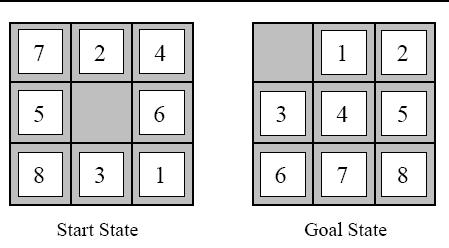
\includegraphics[width=0.47\textwidth]{figs/8-Puzzle.jpg}
	\caption{A randomized 8-puzzle and the goal configuration \cite{fig:puzzle}.}
	\label{fig:puzzle}
\end{figure}

In this paper, we describe the heuristics used by the A* algorithm, detail our experimental approach, including our random board generation method, and then present the results of the comparison in heuristics.

%In this section, you should introduce the reader to the problem you
%are attempting to solve. For example, for the first project: describe
%the $15$-puzzle, and why it's interesting as an A.I. problem. You
%should also cite and briefly describe other related papers that have
%tackled this problem in the past --- things that came up during the
%course of your research. In the AAAI style, citations look like
%\cite{aima} (see the comments in the source file \texttt{intro.tex} to
%see how this citation was produced). Conclude by summarizing how the
%remainder of the paper is organized. \\

%Overall, the aim in this section is context-setting: what is the
%big-picture surrounding the problem you are tackling here?

